\documentclass[11pt]{article}

% fonts
\usepackage[T1]{fontenc}
\usepackage[utf8]{inputenc}
\usepackage[english]{babel}
\usepackage{microtype}
\usepackage{tgschola}
\usepackage{inconsolata}
\usepackage{amsmath}

% images
\usepackage{graphicx}
\usepackage{subfig}
\usepackage{float}
\usepackage{multicol}
\usepackage[ddmmyyyy]{datetime}
\usepackage[a4paper, margin=2cm]{geometry}
\usepackage{wrapfig}

% code listing
\usepackage{minted}
\usemintedstyle{tango}

% sections on new page
\usepackage{titlesec}
\newcommand{\sectionbreak}{\clearpage}
%\setcounter{secnumdepth}{0}

% index and clickable toc
\usepackage{hyperref}
\hypersetup{
	colorlinks,
	citecolor=black,
	filecolor=black,
	linkcolor=black,
	urlcolor=black
}

% bibliography
\usepackage{bookmark}
\usepackage{url}
\usepackage[
	backend=biber,
	style=numeric,
	%citestyle=ieee
]{biblatex}
\usepackage{csquotes}

\addbibresource{bibliography.bib}

% table of content name
%\usepackage[nottoc]{tocbibind}
%\renewcommand{\theHsection}{\thepart.section.\thesection}
%\addto\captionsenglish{% Replace "english" with the language you use
	%\renewcommand{\contentsname}%
	%{\hfill \Huge Table of Content \hfill}%
%}

\begin{document}

	% Title page
	\begin{titlepage}
		\begin{center}

			\vspace*{0.5cm}

			% title
			\Huge
			\textbf{Brain Tumor Detection}

			\vspace{0.8cm}

			% logo
			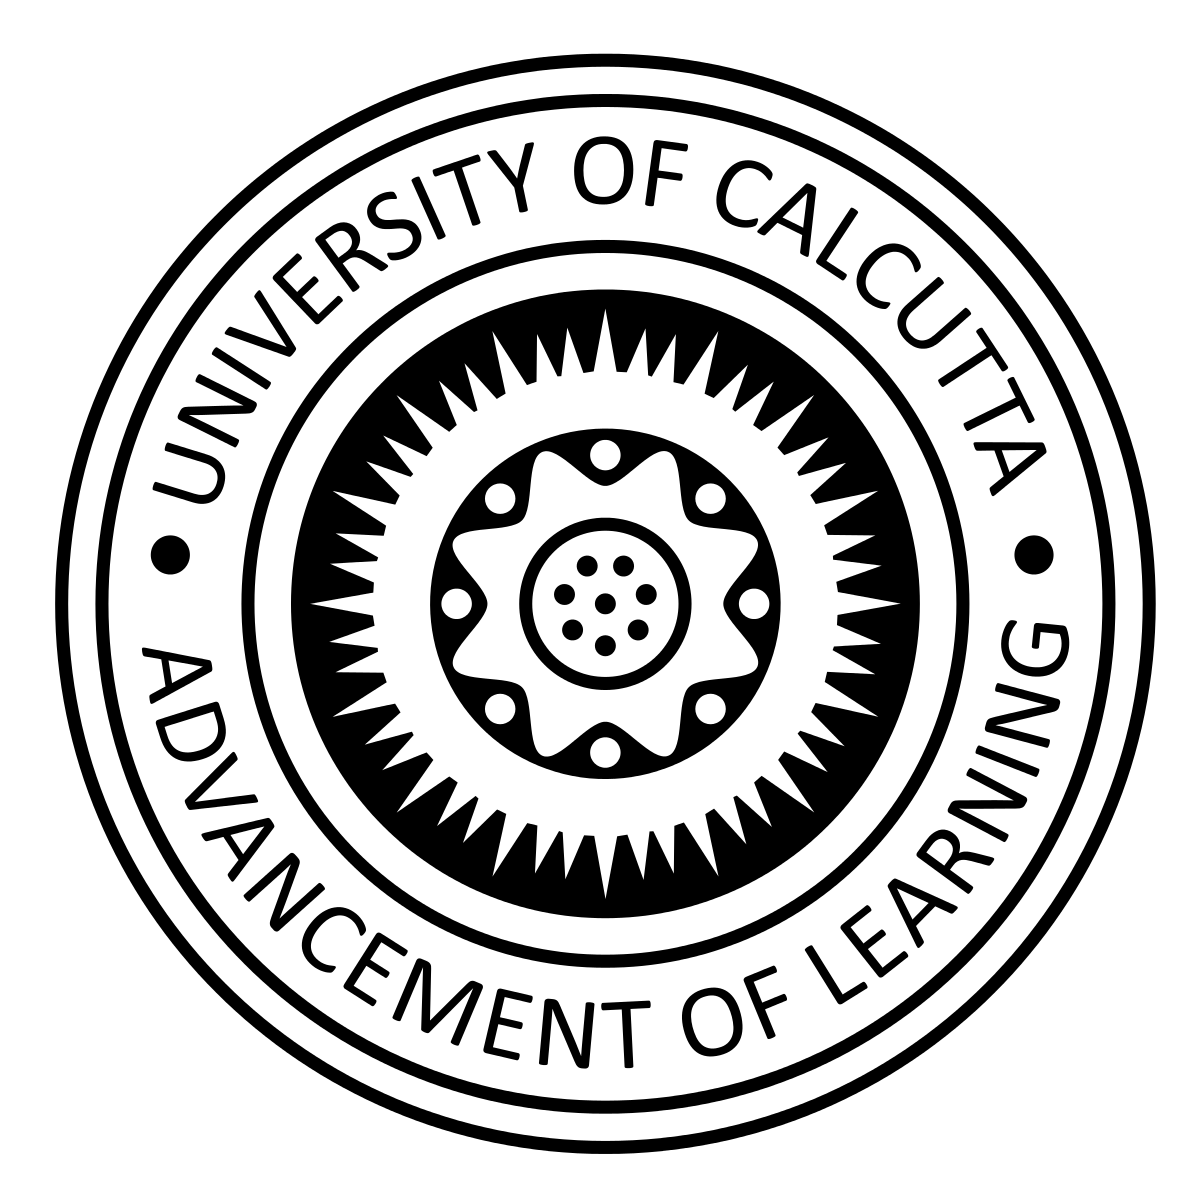
\includegraphics[width=0.4\linewidth]{imgs/cu_logo.png}

			\vspace{1cm}

			\normalsize
			Department of Computer Science\\
			Gurudas College\\
			Calcutta University\\
			\today

			% subtitle
			\vspace{0.5cm}
			\textit{Detection of tumorous cells using machine learning models}

			\vspace{1cm}

			\normalsize
			Submitted in partial fulfillment for the requirements for the
			degree Bachelor of Science (Honors) in Computer Science.

			Academic Year: \textbf{2018-2021}

			\vfill
			% author
			\textbf{Authors}:

			$\bullet$ Shoptorshi \space\space
			$\bullet$ Brahmajit \space\space
			$\bullet$ Rajarshi \space\space
			$\bullet$ Bhargav

			% supervisor
			\vspace{1cm}
			\rule{5cm}{0.4pt}

			\textbf{Supervisor}: Kajari Bhattacharjeee

		\end{center}
	\end{titlepage}

	% certificate page
	\section*{\hfill \Huge Certificate \hfill}
	%\thispagestyle{empty}

	% roman page numbering
	\pagenumbering{roman}

	\begin{center}
		\vspace{1cm}

		% logo
		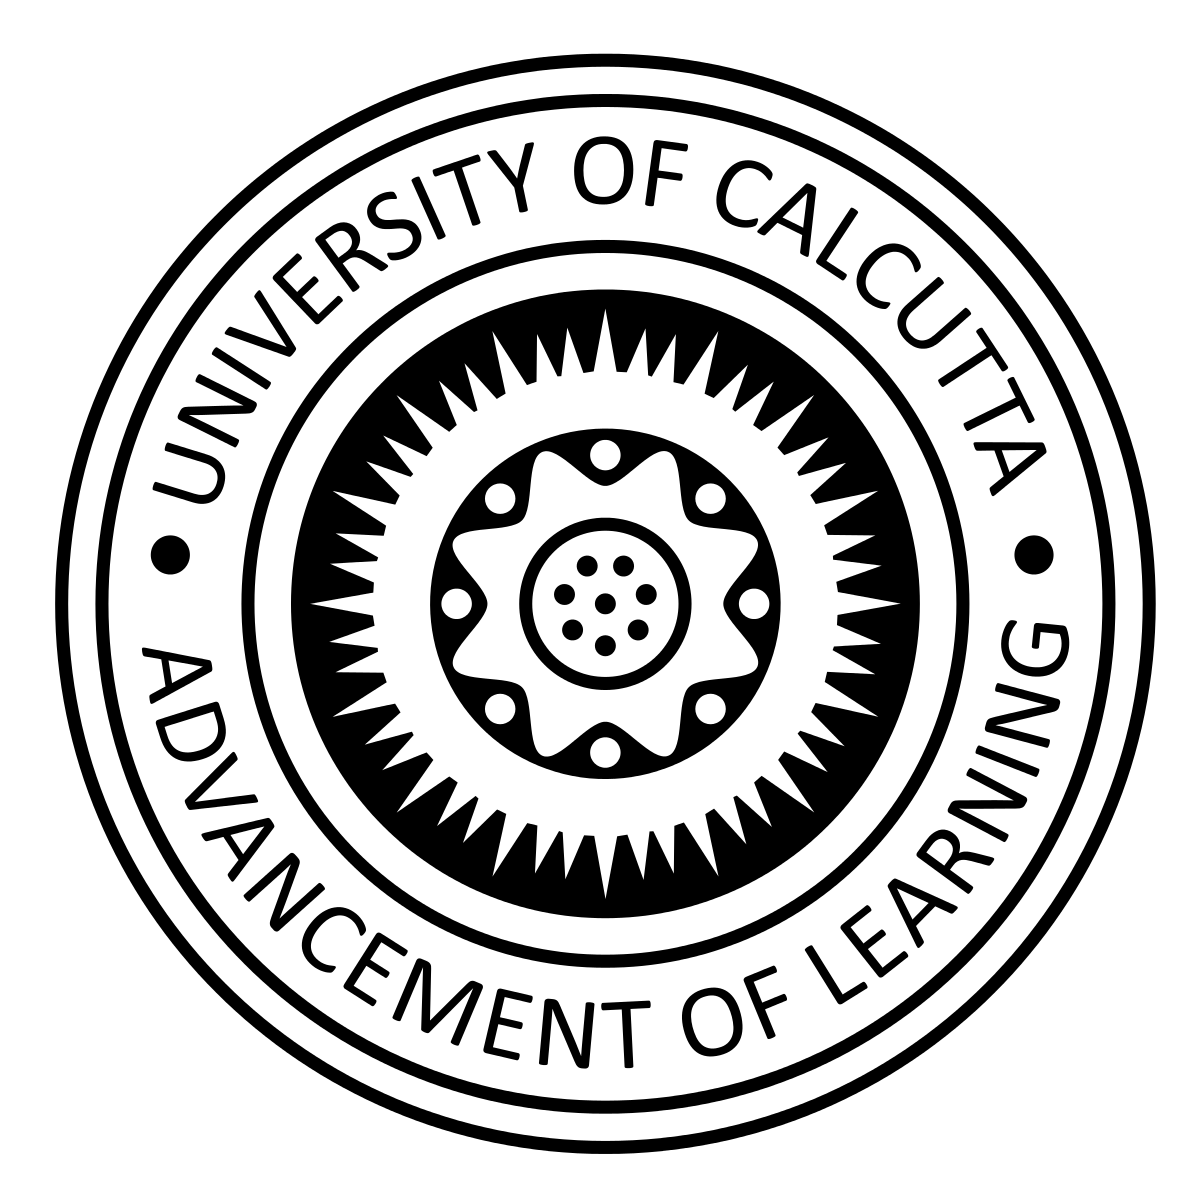
\includegraphics[width=0.3\linewidth]{imgs/cu_logo.png}

		\vspace{1cm}

		\Large
		Department of Computer Science\\
		Gurudas College\\
		Calcutta University\\
	\end{center}

	\vspace{1.8cm}
	This is to certify that the project entitled "Brain tumor detection using
	Machine Learning models" is a bona fide work of \textbf{Shoptorshi},
	\textbf{Brahmajit}, \textbf{Rajarshi} and \textbf{Bhargav} submitted to
	Gurudas College, University of Calcutta; in partial fulfillment of the
	requirement for the award of the degree "Bachelor of Science (Honors)" in
	Computer Science.
	\vfill

	\begin{multicols}{2}

		Supervisor:

		\rule{5cm}{0.4pt}

		\textbf{Kajari Bhattacharjeee}

		\vspace{1cm}

		Department

		Head:

		\rule{5cm}{0.4pt}

		\textbf{Srijeeta Charkraborty}


		\columnbreak

		Principal:

		\rule{5cm}{0.4pt}

		\textbf{Dr. Mausumi Chatterjee}

	\end{multicols}

	\section*{Acknowledgement}
	\label{sec:Acknowledgement}

	\vspace{1cm}

	I would like to express my special thanks of gratitude to our supervisor
	\textbf{Kajari Bhattacharjeee}, teachers of our department \textbf{Sonali
	Gupta} and \textbf{Srijeeta Charkraborty} ( current department head ); as
	well as our principal ma'am \textbf{Dr. Mausumi Chatterjee} who gave us the
	golden opportunity to do this wonderful project on \textit{Brain tumor
	detection}, which has also helped us in doing a lot of research and we came
	to know about many new things.

	We are really thankful to them.

	\vspace{1cm}

	Secondly we would like to thank the incredible authors of the research
	papers in our references/citations for providing us with the information.

	\tableofcontents

	% abstract
	\section[abstract]{Abstract}

	% reverting back to normal page numbering
	\pagenumbering{arabic}

	\thispagestyle{plain}
	\begin{center}
		\Large
		\textbf{Brain Tumor Detection}

		\vspace{0.4cm}
		\large
		Using various machine learning models to detect brain tumor.
	\end{center}

	Tumors are cancerous or non-cancerous mass or growth of abnormal cells in
	brain. Tumors can start in brain, or cancer elsewhere in the body can spread
	to brain. There are many way to control the occurrence of these abnormal
	cells. A tumor can be denoted as a malformed mass of tissues wherein the
	cells multiply abruptly and ceaselessly, that is there is no control over
	the growth of the cells.

	The process of Image segmentation is adopted for extracting abnormal tumor
	region within the brain. In the MRI (magnetic resonance image), segmentation
	of brain tissue holds very significant in order to identify the presence of
	outlines concerning the brain tumor. There is abundance of hidden
	information in stored in the Health care sector. With appropriate use of
	accurate data mining classification techniques, early prediction of any
	disease can be effectively performed.

	The project examines list of risk factors that are being traced out in brain
	tumor surveillance systems. Also the method proposed assures to be highly
	efficient and precise for brain tumor detection, classification and
	segmentation. To achieve this precise automatic or semi-automatic methods
	are needed. The project proposes an automatic segmentation method that
	relies upon \textit{ CNN (Convolution Neural Networks) }, \textit{ VGG 16 }
	and \textit{ Resent 50 }, determining small 7 x 7 kernels. By incorporating
	this single technique, segmentation and classification is accomplished. CNN
	(a ML technique) from NN (Neural Networks)wherein it has layer based for
	results classification.

	Various levels involved in the proposed mechanisms are:

	\begin{enumerate}
		\item \textbf{ Data collection }
		\item \textbf{ Pre-processing }
		\item \textbf{ Average filtering }
		\item \textbf{ segmentation }
		\item \textbf{ feature extraction }
		\item \textbf{CNN (or any other model) via classification and identification. By
			utilizing the DM (data mining) techniques, significant relations and
			patterns from the data can be extracted. The techniques of ML
			(machine learning) and Data mining are being effectively employed
			for brain tumor detection and prevention at an early stage.}
	\end{enumerate}

	\section[introduction]{Introduction}
	\subsection[domain description]{Domain Description}

	\begin{enumerate}
		\item \textbf{Neurological Examination}: It is a series of test to
			measures the function of the patients nervous system and also
			his/her physical and mental alertness.
		\item \textbf{Machine Learning}: Machine learning approaches address
			these problems by mainly using hand-crafted features (or pre-defined
			features). As an initial step in this kind of segmentation, the key
			information is extracted from the input image using some feature
			extraction algorithm, and then a discriminative model is trained to
			recognize the tumor from normal tissues. The designed machine
			learning techniques generally employ hand-crafted features with
			various classifiers, such as random forest, support vector machine
			(SVM), fuzzy clustering. The designed methods and features
			extraction algorithms have to extract features, edge-related
			details, and other necessary information—which is time-consuming.
			Moreover, when boundaries between healthy tissues and tumors are
			fuzzy/vague, these methods demonstrate poorer performances.
		\item \textbf{Brain Scan}: Brain scan is a picture of the internal
			structure of the brain. A specialized machine takes a scan in the
			same way as a digital camera takes a photograph. Using computer
			technology, a scan compiles an image of the brain by photographing
			it from various angles. Some types of scan uses contrast agent (or
			contrast dye), which helps the doctor to see the difference between
			normal and abnormal brain tissues.

			MRI (Magnetic Resonance Imaging): It is a scanning device that uses
			magnetic field and computer to capture images of the brain on films.
			It does not use x-rays. It provides pictures from various planes,
			which permits doctor to create a three-dimensional image of the
			tumor. The MRI detects signals emitted from normal and abnormal
			tissues, providing clear images of almost all tumors.
	\end{enumerate}

	\subsection[motivation]{Motivation}
	The motivation is to develop a software with better segmentation capability
	for use in medical imaging to detect diseases like brain tumor. Image
	segmentation has been identified as the key problem of medical image
	analysis and remains a popular and challenging area of research. Image
	segmentation is increasingly used in many clinical and research applications
	to analyze medical imaging datasets; which motivated us to present a
	snapshot of dynamically changing field of medical image segmentation.

	CT (Computed Tomography), MRI (Magnetic Resonance Imaging), PET (Positron
	Emission Tomography) etc. generates a large amount of image information.
	With the improved technology, not only does the size and resolution of the
	images grow but also the number of dimensions increases. In the future, we
	would like to have algorithms which can automatically detect diseases,
	lesions and tumors, and highlight their locations in the large pile of
	images.

	The motivation of this work is to increase patient safety by providing
	better and more precise data for medical decision.

	\subsection[scope of work]{Scope of Work}
	\subsubsection[deliverables]{Deliverables}
	\begin{itemize}
		\item Working program to take an MRI scan as input and predict presence
			of tumorous cells with $\geq 90\%$ accuracy.
	\end{itemize}

	\subsubsection[scope]{Scope}
	\begin{itemize}
		\item The working program has external dependencies ( libraries ) and
			it's expected to have a them installed for the program to work.
	\end{itemize}

	\subsubsection[timeline]{Timeline}
	\begin{itemize}
		\item \textbf{April 27, 2021} Project Assigned
		\item \textbf{May 2, 2021} Project finalized by supervisor, and group is
			divided into groups of two.
		\item \textbf{May 3, 2021} Data collection started.
		\item \textbf{May 12, 2021} Project Repository created and coding is
			started.
		\item \textbf{July 7, 2021} Coding is finished, documentation is
			started.
		\item \textbf{Just 21, 2021} Documentation complete.
	\end{itemize}

	\subsubsection[reports]{Reports}
	\begin{itemize}
		\item Constantly updating and pushing code to repository.
		\item Both teams staying in touch with each other to keep up with each
			others progress.
		\item Report back to supervisor every once a week.
	\end{itemize}

	\section[background]{Background}
		Natarajan \cite{bac1} proposed brain tumor detection method for MRI brain
	images. The MRI brain images are first preprocessed using median filter,
	then segmentation of image is done using threshold segmentation and
	morphological operations are applied and then finally, the tumor region is
	obtained using image subtraction technique. This approach gives the exact
	shape of tumor in MRI brain image. Joshi \cite{bac2} proposed brain tumor
	detection and classification system in MR images by first extracting the
	tumor portion from brain image, then extracting the texture features of the
	detected tumor using Gray Level Co-occurrence Matrix (GLCM) and then
	classified using neuro-fuzzy classifier. Amin and Mageed \cite{bac3}
	proposed neural network and segmentation base system to automatically detect
	the tumor in brain MRI images. The Principal Component Analysis (PCA) is
	used for feature extraction and then Multi-Layer Perceptron (MLP) is used
	classify the extracted features of MRI brain image. The average recognition
	rate is 88.2\% and peak recognition rate is 96.7\%. Sapra \cite{bac4}
	proposed image segmentation technique to detect brain tumor from MRI images
	and then Probabilistic Neural Network (PNN) is used for automated brain
	tumor classification in MRI scans. PNN system proposed handle the process of
	brain tumor classification more accurately. Suchita and Lalit \cite{bac5}
	proposed unsupervised neural network learning technique for classification
	of brain MRI images. The MRI brain images are first preprocessed which
	include noise filtering, edge detection, then the tumor is extracted using
	segmentation. The texture features are extracted using Gray-Level
	Co-occurrence Matrix(GLCM) and then Self-Organizing Maps (SOM) are used to
	classify the brain as normal or abnormal brain, that is, whether it contain
	tumor or not. Rajeshwari and Sharmila \cite{bac6} proposed preprocessing
	techniques which are used to improve the quality of MRI image before using
	it into an application. The average, median and wiener filters are used for
	noise removal and interpolation based Discrete Wavelet Transform (DWT)
	technique is used for resolution enhancement. The Peak Signal to Noise Ratio
	(PSNR) is used for evaluation of these techniques.

	George and Karnan \cite{George2012MRIBI} proposed MRI image enhancement
	technique based on Histogram Equalization and Center Weighted Median (CWM)
	filter as they are used to enhance the MRI image more effectively. Daljit
	Singh et \cite{Funmilola2015ClassificationOA} proposed a hybrid technique
	for automatic classification of MRI images by first extracting the features
	using Principal Component Analysis (PCA) and Gray-Level Co-occurrence
	Matrix(GLCM) and then extracted features are fed as an input to Support
	Vector Machine(SVM) classifier which classifies the brain image as normal or
	abnormal. Gadpayleand and Mahajani \cite{9074375} proposed brain tumour
	detection and classification system. The tumor is extracted using
	segmentation and then texture features are extracted using GLCM and finally
	the BPNN and KNN classifiers are used to classify the MRI brain image into
	normal or abnormal brain. The accuracy is 70\% using KNN classifier and
	72.5\% by using BPNN classifier. Shasidhar et al. in \cite{article} proposed
	modified Fuzzy C-Means (FCM) algorithm for MR brain tumor detection. The
	texture features are extracted from brain MR image and then modified FCM
	algorithm is used for brain tumor detection. The average speed-ups of as
	much as 80 times a traditional FCM algorithm is obtained using the modified
	FCM algorithm. The modified FCM algorithm is a fast alternative to the
	traditional FCM technique.  Rajesh and Malar \cite{inproceedings} proposed
	brain MR image classification based on Rough set theory and feed-forward
	neural network classifier. The features are extracted from MRI images using
	Rough set theory. The selected features are fed as input to Feed Forward
	Neural Network classifier which differentiate between normal and abnormal
	brain and the accuracy of about 90\% is obtained.

	Ramteke and Monali \cite{article2} proposed automatic classification of
	brain MR images in two classes Normal and Abnormal based on image features
	and automatic abnormality detection. The Statistical texture feature set is
	obtained from normal and abnormal images and then KNN classifier is used for
	classifying image. The KNN obtain 80\% classification rate.  Xuan and Liao
	\cite{4297123} proposed statistical structure analysis based tumor
	segmentation technique. The intensity-based, symmetry-based and texture-
	based features are extracted from MR image. Then, classification technique
	using AdaBoost is used to classify the MR image into normal tissues and
	abnormal images. The average accuracy of about 96.82\% is achieved. Othman
	et al. in \cite{5730335} proposed Probabilistic neural network technique for
	brain tumor classification. Firstly, the features are extracted using the
	principal component analysis (PCA) and the classification is performed using
	Probabilistic Neural Network (PNN).  Ibrahim et al. in \cite{inproceedings2}
	proposed Neural Network technique for the classification of the magnetic
	resonance human brain images. The features are extracted using principal
	Component Analysis (PCA) and then Back- Propagation Neural Network is used
	as a classifier to classify MRI brain images as normal or abnormal. The
	classification accuracy of about 96.33\% is obtained. Jafari and Shafaghi
	\cite{article3} proposed a hybrid approach for brain tumor detection in MR
	images based on Support Vector Machines(SVM). The texture and intensity
	features are used. The accuracy of about 83.22\% is achieved and is more
	robust.

	Thus from extensive literature survey we found that most of the current
	brain tumor detection system uses texture, symmetry and intensity as
	features. Texture features are important property of brain as texture
	perception has a very important aspect in the human visual system of
	recognition and interpretation \cite{article4}. Here, we propose extracting
	texture features like energy, contrast, correlation, Homogenity
	\cite{6524466}. Gray Level Co-occurrence Matrix is used for extraction of
	texture features.

	Further we propose the use of ML algorithms to overcome the drawbacks of
	traditional classifiers. We investigate and compare the performance of three
	machine learning models namely CNN, VGG-16 and Resnet-50 in this work. Since
	these ML models are found to perform well in most of the pattern
	classification tasks. Neural networks are useful as they can learn complex
	mappings between input and output. They are capable of solving much more
	complicated classification tasks.


	\section[methodology]{Methodology}

	As per literature survey, it was found that automated  brain  tumor
	detection  is  very  necessary  as  high accuracy is needed when human life
	is involved.  Automated detection of tumor in MR images involves feature
	extraction and  classification  using  machine  learning  algorithm.  In
	this paper, a system to automatically detect tumor in MR images is proposed
	as shown in Figure~\ref{Proposed Methodology}

	\begin{figure}[h]
		\centering
		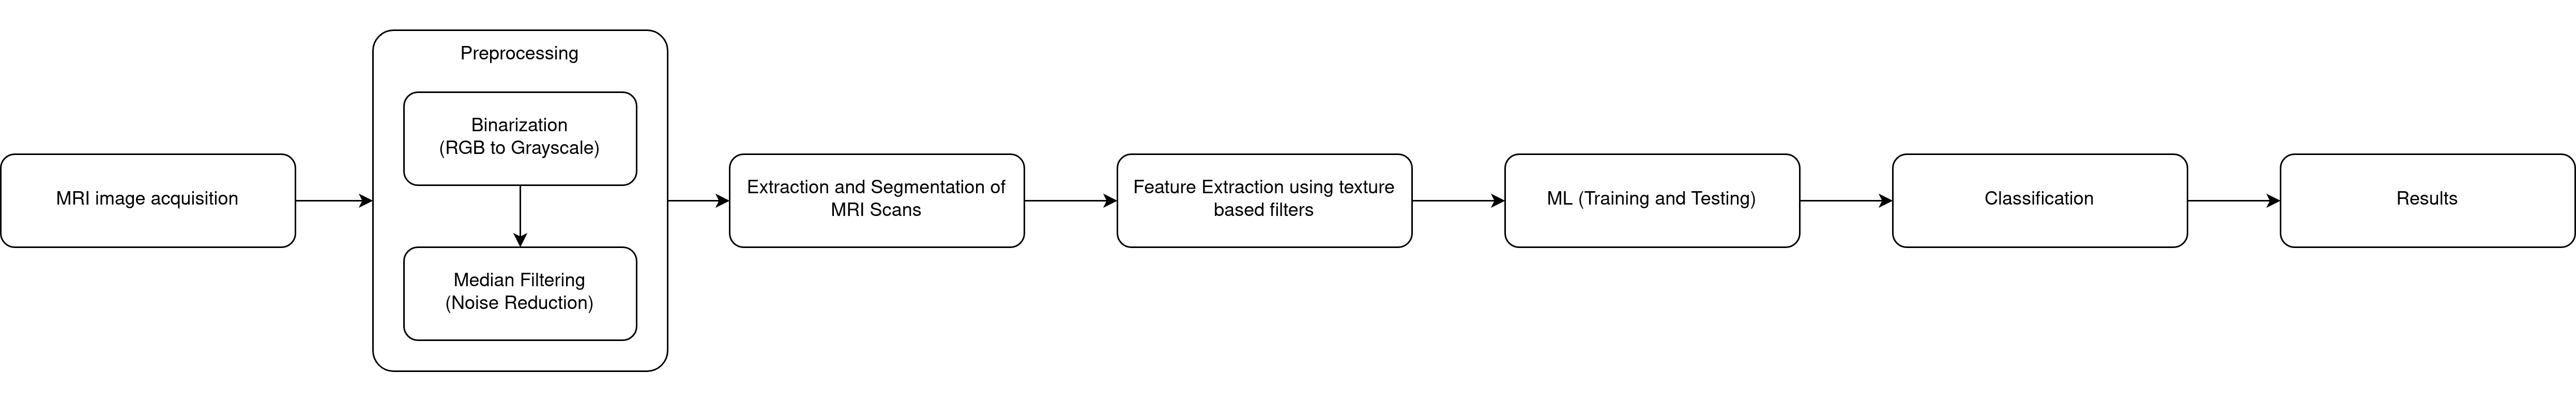
\includegraphics[width=1\linewidth]{imgs/methodology}
		\caption{Proposed Methodology}%
		\label{Proposed Methodology}
	\end{figure}

	\subsection{Image Acquisition}%
	\label{sub:Image Acquisition}

	The MRI brain images are acquired and are
	given as input to pre-processing stage. The sample brain MR images are shown
	in Figure~\ref{MRIScans}.

	\begin{figure}[H]
		\centering
		\subfloat[MRI scan shown no presence of tumor]
		{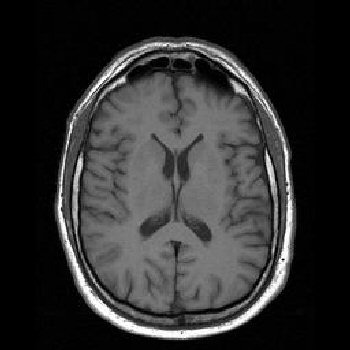
\includegraphics[width=0.4\linewidth]
		{imgs/pred1.jpg}\label{scan2}}
		\hspace{0.5cm}
		\subfloat[MRI scan of a tumorous cell]
		{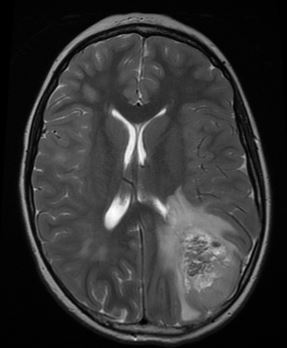
\includegraphics[width=0.3\linewidth]
		{imgs/Y100.JPG}\label{scan1}}
		\caption{MRI Scans}
		\label{MRIScans}
	\end{figure}

	\subsection{Preprocessing}%
	\label{sub:Preprocessing}

	Preprocessing is needed as it provides improvement
	in image data which  enhances some of the image features which are important
	for further processing. The  pre-processing steps that are applied to MR
	image are as follows:

	\begin{enumerate}
		\item The  RGB  MR    image  is  converted  to  gray  scale image  and
			then  median  filter  is  applied  for  noise  removal from brain MR
			images as shown in Figure~\ref{smooted image}. The noise is to removed for further
			processing as high accuracy is needed.

		\item Then  edges  are  detected  from  filtered  image  using canny
			edge  detection  as  shown  in  Figure~\ref{edge detection}.  The  edge detected
			image is needed for segmentation of  the image

		\item Then  watershed  segmentation  is  done  for  finding the
			location  of  the  tumor  in  the  brain  image  as  shown  in
			Figure~\ref{segmentation}. Segmentation is  the process of dividing  an image into
			multiple segments. The aim of segmentation is to change
			representation  of    image  into  something  which  is more  easy
			to  analyze.  The result  of  watershed  segmentation is  label
			image.    In  label  image,  all  the  different  objects identified
			will  have  different  pixel  values  ,  all  the  pixels  of first
			object  will have value 1, all the pixels of second object will have
			value 2 and so on.
	\end{enumerate}


	\begin{figure}[H]
		\centering
		\subfloat[Original Image]
		{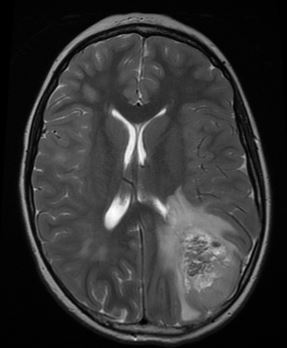
\includegraphics[width=0.2\linewidth]
		{imgs/Y100.JPG}\label{original}}
		\hspace{0.5cm}
		\subfloat[Filtered Imaage]
		{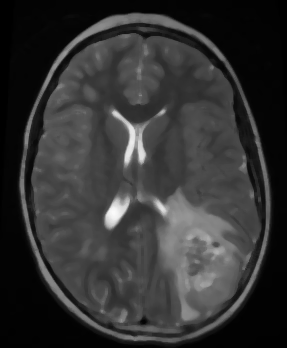
\includegraphics[width=0.2\linewidth]
		{imgs/median_filtering.png}\label{smooted image}}
		\hspace{0.5cm}
		\subfloat[Edge Detection]
		{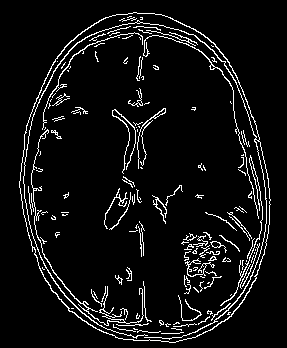
\includegraphics[width=0.2\linewidth]
		{imgs/edges_detection.png}\label{edge detection}}
		\hspace{0.5cm}
		\subfloat[Segmentation]
		{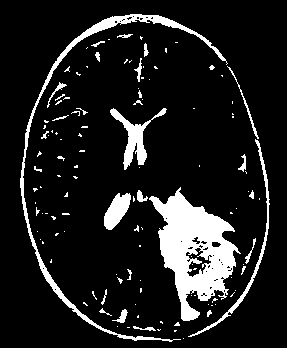
\includegraphics[width=0.2\linewidth]
		{imgs/segmentation.png}\label{segmentation}}
		\caption{preprocessing operations}
		\label{Preprocessing Operations}
	\end{figure}

	\subsection{Feature Extraction}%
	\label{sub:Feature Extraction}

	When input to an algorithm is very large and
	redundant to be processed, it is transformed into reduced representative set
	of features called feature vector. Transformation of input data into set of
	features is called feature extraction. In this step, the important features
	needed for image classification are extracted. The segmented brain MR image
	is used and texture features are extracted from the segmented image which
	shows the texture property of the image. These features are extracted using
	Gray Level Co-occurrence Matrix (GLCM) as it is robust method with high
	performance.

	The GLCM features are extracted as follows:

	\begin{enumerate}
		\item Energy: It gives a measure of textural uniformity, that is, measure
			of pixel pair repetitions.

			\begin{equation}
				E = \sum^{N_g - 1}_{i=0} \sum^{N_g - 1}_{j=0} p(i, j)^2 \
				\textnormal{ here, range = [0, 1] }
			\end{equation}

		\item Contrast: It gives a measure of intensity contrast between a pixel
			and its neighbor over the whole image.

			\begin{equation}
				Con = \sum^{N_g -1}_{n=0} n^2 \sum^{N_g -1}_{i=0} \sum^{N_g
				-1}_{j=0} p(i,j)^2 \
				\textnormal{ here, range = [0, 1] }
			\end{equation}

		\item Correlation: It gives a measure of how correlated a pixel to its
			neighbor over the whole image.

			\begin{equation}
				C = \frac{1}{\sigma^x \sigma^y}
				\sum^{N_g - 1}_{i=0} \sum^{N_g -1}_{j=0} (i,j) p(i,j)^2
				- \mu_x \mu_y \ \textnormal{here, range = [-1, 1]}
			\end{equation}

		\item Homogeneity: It gives a measure of closeness of distribution of
			elements in GLCM to GLCM diagonal.

			\begin{equation}
				H = \sum^{N_g -1}_{i=0} \sum^{N_g -1}_{j=0}
				\frac{p(i,j)}{1 + \pmod{i,j}}
				\ \textnormal{here, range = [0, 1]}
			\end{equation}
	\end{enumerate}

	\subsection{Classification}%
	\label{sub:Classification}

	The Machine learning algorithms are used for
	classification of MR brain image either as normal or abnormal.  The major
	aim of ML algorithms is to automatically learn and make intelligent
	decisions. The feature set formed by above specified method was applied to
	Multi-Layer Perceptron (MLP) and Naive Bayes for classification.  MLP is
	a feed forward artificial neural network model that maps sets of input data
	into a set of appropriate output. It is known as feed forward because it
	does not contain any cycles and network output depends only on the current
	input instance. In MLP, each node is a neuron with a nonlinear activation
	function. It is based on supervised learning technique. Learning take place
	by changing connection weights after each piece of data is processed, based
	on the amount of error in the target output as compared to the expected
	result. The goal of the learning procedure is to minimize error by improving
	the current values of the weight associated with each edge. Because of this
	backward changing process of the weights, model is named as
	back-propagation.

	Naive bayes is a supervised learning as well as statistical method for
	classification. It is simple probabilistic classifier based on Bayes
	theorem. It assumes that the value of a particular feature is unrelated to
	the presence or absence of any other feature. The prior probability and
	likelihood are calculated in order to calculate the posterior probability.
	The method of maximum posterior probability is used for parameter
	estimation. This method requires only a small amount of training data to
	estimate the parameters which are needed for classification. The time taken
	for training and classification is less.

	For classification three models are used; \textbf{CNN}, \textbf{VGG 16} and
	\textbf{Resnet 50}.

	\subsection{Convolutional Neural Network}%
	\label{sub:Convolutional Neural Network}

	CNN or Convolutional Neural Network a class of artificial neural network,
	most commonly applied to analyze visual imagery.They are also known as
	shift invariant or space invariant artificial neural networks (SIANN), based
	on the shared-weight architecture of the convolution kernels or filters that
	slide along input features and provide translation equivariant responses
	known as feature maps. Counter-intuitively, most convolutional neural
	networks are only equivariant, as opposed to invariant, to translation.
	They have applications in image and video recognition, recommender
	systems, image classification, image segmentation, medical image
	analysis, natural language processing, brain-computer interfaces, and
	financial time series.

	\begin{figure}[h]
		\centering
		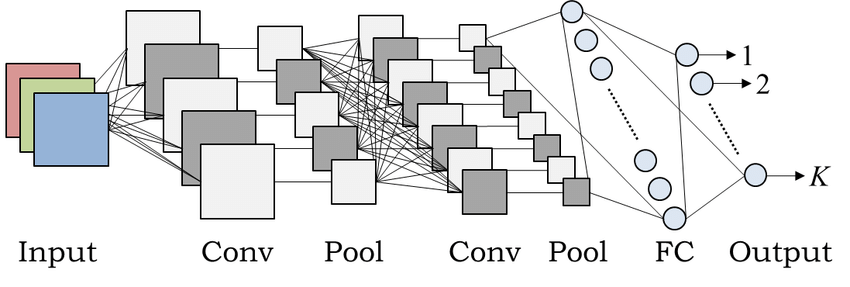
\includegraphics[width=0.8\linewidth]{imgs/cnn_arch.png}
		\caption{CNN architecture}%
		\label{CNN Architecture}
	\end{figure}

	\subsubsection{Architecture}

	A convolutional neural network consists of an input layer, hidden layers and
	an output layer. In any feed-forward neural network, any middle layers are
	called hidden because their inputs and outputs are masked by the activation
	function and final convolution. In a convolutional neural network, the
	hidden layers include layers that perform convolutions. Typically this
	includes a layer that performs a dot product of the convolution kernel with
	the layer's input matrix.  This product is usually the Frobenius inner
	product, and its activation function is commonly ReLU. As the convolution
	kernel slides along the input matrix for the layer, the convolution
	operation generates a feature map, which in turn contributes to the input of
	the next layer. This is followed by other layers such as pooling layers,
	fully connected layers, and normalization layers \cite{covnet_arch}.

	\textbf{Convolutional Layer}:
	In a CNN, the input is a tensor with a shape: (number of inputs) x (input
	height) x (input width) x (input channels). After passing through a
	convolutional layer, the image becomes abstracted to a feature map, also
	called an activation map, with shape: (number of inputs) x (feature map
	height) x (feature map width) x (feature map channels). A convolutional
	layer within a CNN generally has the following attributes:

	\begin{itemize}
		\item Convolutional filters/kernels defined by a width and height (hyper-parameters).
		\item The number of input channels and output channels
			(hyper-parameters). One layer's input channels must equal the number
			of output channels (also called depth) of its input.
		\item Additional hyperparameters of the convolution operation, such as:
			padding, stride, and dilation.
	\end{itemize}

	Convolutional layers convolve the input and pass its result to the next
	layer. This is similar to the response of a neuron in the visual cortex to a
	specific stimulus.

	\textbf{Pooling Layer}:
	Convolutional networks may include local and/or global pooling layers along
	with traditional convolutional layers. Pooling layers reduce the dimensions
	of data by combining the outputs of neuron clusters at one layer into a
	single neuron in the next layer. Local pooling combines small clusters,
	tiling sizes such as 2 x 2 are commonly used. Global pooling acts on all the
	neurons of the feature map. There are two common types of pooling in popular
	use: max and average. Max pooling uses the maximum value of each local
	cluster of neurons in the feature map, while average pooling takes the
	average value.

	\textbf{ReLU Layer}:

	ReLU is the abbreviation of rectified linear unit, which applies the
	non-saturating activation function
	\begin{equation}
		f ( x ) = \max ( 0 , x )
	\end{equation}

	.It effectively removes
	negative values from an activation map by setting them to zero. It
	introduces nonlinearities to the decision function and in the overall
	network without affecting the receptive fields of the convolution layers.

	Other functions can also be used to increase nonlinearity, for example the
	saturating hyperbolic tangent
	\begin{equation}
	f(x)=\tanh(x)
	f(x) = | \tanh (x) |
	\end{equation}
	and the
	sigmoid function

	\begin{equation}
		\sigma(x) = (1+e^{-x})^{-1}
	\end{equation}

	ReLU is often preferred to other functions because it trains the neural network several
	times faster without a significant penalty to generalization accuracy
	 \cite{relu_layer}.

	\textbf{Fully Connected Layer}

	After several convolutional and max pooling layers, the final classification
	is done via fully connected layers. Neurons in a fully connected layer have
	connections to all activations in the previous layer, as seen in regular
	(non-convolutional) artificial neural networks. Their activations can thus
	be computed as an affine transformation, with matrix multiplication followed
	by a bias offset (vector addition of a learned or fixed bias term).

	\textbf{Loss Layer}

	The "loss layer", or "loss function", specifies how training penalizes the
	deviation between the predicted output of the network, and the true data
	labels (during supervised learning). Various loss functions can be used,
	depending on the specific task.

	The Softmax loss function is used for predicting a single class of K
	mutually exclusive classes. Sigmoid cross-entropy loss is used for
	predicting K independent probability values is $[0, 1]$.  Euclidean loss is
	used for regressing to real-valued labels $(- \infty, \infty)$.

	\textbf{Receptive field}

	In neural networks, each neuron receives input from some number of locations
	in the previous layer. In a convolutional layer, each neuron receives input
	from only a restricted area of the previous layer called the neuron's
	receptive field. Typically the area is a square (e.g. 5 by 5 neurons).
	Whereas, in a fully connected layer, the receptive field is the entire
	previous layer. Thus, in each convolutional layer, each neuron takes input
	from a larger area in the input than previous layers. This is due to
	applying the convolution over and over, which takes into account the value
	of a pixel, as well as its surrounding pixels. When using dilated layers,
	the number of pixels in the receptive field remains constant, but the field
	is more sparsely populated as its dimensions grow when combining the effect
	of several layers.

	\textbf{Weights}

	Each neuron in a neural network computes an output value by applying a
	specific function to the input values received from the receptive field in
	the previous layer. The function that is applied to the input values is
	determined by a vector of weights and a bias (typically real numbers).
	Learning consists of iteratively adjusting these biases and weights.

	The vector of weights and the bias are called filters and represent
	particular features of the input (e.g., a particular shape). A
	distinguishing feature of CNNs is that many neurons can share the same
	filter. This reduces the memory footprint because a single bias and a single
	vector of weights are used across all receptive fields that share that
	filter, as opposed to each receptive field having its own bias and vector
	weighting.

	\subsection{VGG 16}

	VGG 16 is is a significantly more accurate ConvNet architecture, which not
	only achieve state-of-the-art accuracy on ILSVRC classification and
	localisation tasks, but are also applicable to other image recognition
	datasets, where they achieve excellent performance even when used as a part
	of a relatively simple pipelines (e.g. deep features classified by a linear
	SVM without fine-tuning) \cite[1]{simonyan2015deep}.

	\subsubsection{Architecture}
	\label{sssec:vgg arch}

	\begin{wrapfigure}{r}{0.5\textwidth}
		\begin{center}
			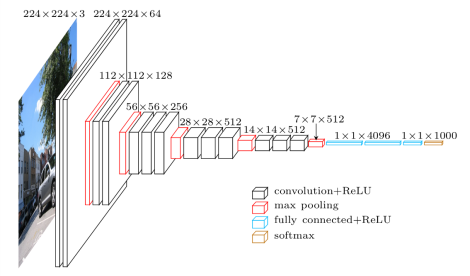
\includegraphics[ width=0.5\textwidth ]{imgs/vgg16_arch.png}
		\end{center}
		\caption{VGG Architecture}
	\end{wrapfigure}

	During training, the input to our ConvNets is a fixed-size 224 × 224 RGB
	image. The only pre- processing we do is subtracting the mean RGB value,
	computed on the training set, from each pixel.  The image is passed through
	a stack of convolutional (conv.) layers, where we use filters with a very
	small receptive field: 3 × 3 (which is the smallest size to capture the
	notion of left/right, up/down, center). In one of the configurations we also
	utilise 1 × 1 convolution filters, which can be seen as a linear
	transformation of the input channels (followed by non-linearity). The
	convolution stride is fixed to 1 pixel; the spatial padding of conv. layer
	input is such that the spatial resolution is preserved after convolution,
	i.e. the padding is 1 pixel for 3 × 3 conv. layers. Spatial pooling is
	carried out by five max-pooling layers, which follow some of the conv.
	layers (not all the conv. layers are followed by max-pooling). Max-pooling
	is performed over a 2 × 2 pixel window, with stride 2.

	A stack of convolutional layers (which has a different depth in different
	architectures) is followed by three Fully-Connected (FC) layers: the first
	two have 4096 channels each, the third performs 1000- way ILSVRC
	classification and thus contains 1000 channels (one for each class). The
	final layer is the soft-max layer. The configuration of the fully connected
	layers is the same in all networks.

	All hidden layers are equipped with the rectification (ReLU) non-linearity.
	We note that none of our networks (except for one) contain Local Response
	Normalisation (LRN) normalisation: as will be shown in Sect. 4, such
	normalisation does not improve the performance on the ILSVRC dataset, but
	leads to increased memory con- sumption and computation time.
	\cite[1]{simonyan2015deep}

	\subsubsection{Configuration}

	The ConvNet configurations, evaluated in this paper, are outlined in
	Figure~\ref{fig:vgg16_conf}, one per column. In the following we will refer
	to the nets by their names (A–E).  All configurations follow the generic
	design presented in Section~\ref{sssec:vgg arch} and differ only in the
	depth: from 11 weight layers in the network A (8 conv. and 3 FC layers) to
	19 weight layers in the network E (16 conv. and 3 FC layers). The width of
	conv. layers (the number of channels) is rather small, starting from 64 in
	the first layer and then increasing by a factor of 2 after each max-pooling
	layer, until it reaches 512.
	\cite[3]{simonyan2015deep}

	\begin{figure}[h]
		\centering
		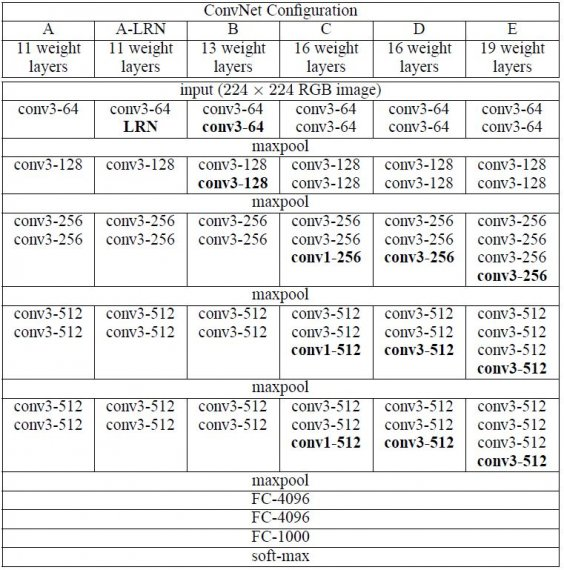
\includegraphics[width=\linewidth]{imgs/vgg16_conf}
		\caption{VGG16 configuration}%
		\label{fig:vgg16_conf}
	\end{figure}

	\subsection{ResNet 50}%
	\label{sub:ResNet 50}

	\subsubsection{Residual Learning}

	\begin{wrapfigure}{r}{0.5\textwidth}
		\begin{center}
			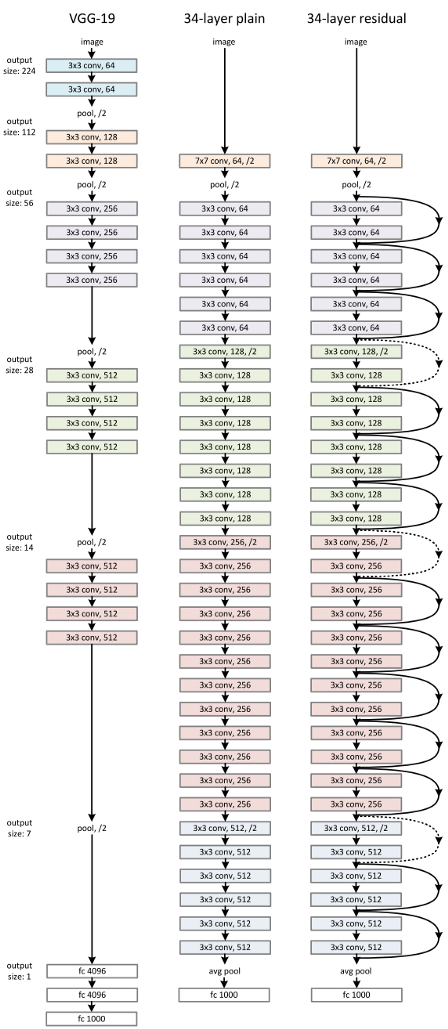
\includegraphics[ width=0.5\textwidth ]{imgs/resnet_arch2.png}
		\end{center}
		\caption{Resnet Architecture}
	\end{wrapfigure}

	Let us consider $H(x)$ as an underlying mapping to be fit by a few stacked
	layers (not necessarily the entire net), with $x$ denoting the inputs to the
	first of these layers. If one hypothesizes that multiple nonlinear layers
	can asymptotically approximate complicated functions, then it is equivalent
	to hypothesize that they can asymptotically approximate the residual
	functions, i.e., $H(x) - x$ (assuming that the input and output are of the
	same dimensions). So rather than expect stacked layers to approximate $H(x)$
	, we explicitly let these layers approximate a residual function
	\begin{equation}
		F(x) = H(x) - x
	\end{equation}
	The original function thus becomes $F(x) + x$. Although both forms should be
	able to asymptot- ically approximate the desired functions (as
	hypothesized), the ease of learning might be different \cite[3]{he2015deep}.

	\subsubsection{Network Architecture}

	The plain/residual network was tested as follows:

	\textbf{Plain Network}

	Our plain baselines are mainly inspired by the philosophy of VGG nets.  The
	convolutional layers mostly have 3×3 filters and follow two simple design
	rules:

	\begin{enumerate}
		\item for the same output feature map size, the layers have the same
			number of filters
		\item if the feature map size is halved, the number of filters is
			doubled so as to preserve the time complexity per layer.
	\end{enumerate}

	We perform downsampling directly by convolutional layers that have a stride
	of 2. The network ends with a global average pooling layer and a 1000-way
	fully-connected layer with softmax. The total number of weighted layers are
	34.  It is worth noticing that our model has fewer filters and lower
	complexity than VGG nets. Our 34-layer baseline has 3.6 billion FLOPs
	(multiply-adds), which is only 18\% of VGG-19 (19.6 billion FLOPs)
	\cite[3]{he2015deep} .

	\textbf{Residual Network}
	Based on the above plain network, we insert shortcut connections which turn
	the network into its counterpart residual version. The identity shortcuts
	can be directly used when the input and output are of the same dimensions.
	When the dimensions increase, we consider two options:
	\begin{enumerate}
		\item The shortcut still performs identity mapping, with extra zero
			entries padded for increasing dimensions. This option introduces no
			extra parameter
		\item The projection shortcut is used to match dimensions (done by 1×1
			convolutions).
	\end{enumerate}
	For both options, when the shortcuts go across feature maps of two sizes,
	they are performed with a stride of 2 \cite[4]{he2015deep} .

	\begin{figure}[h]
		\centering
		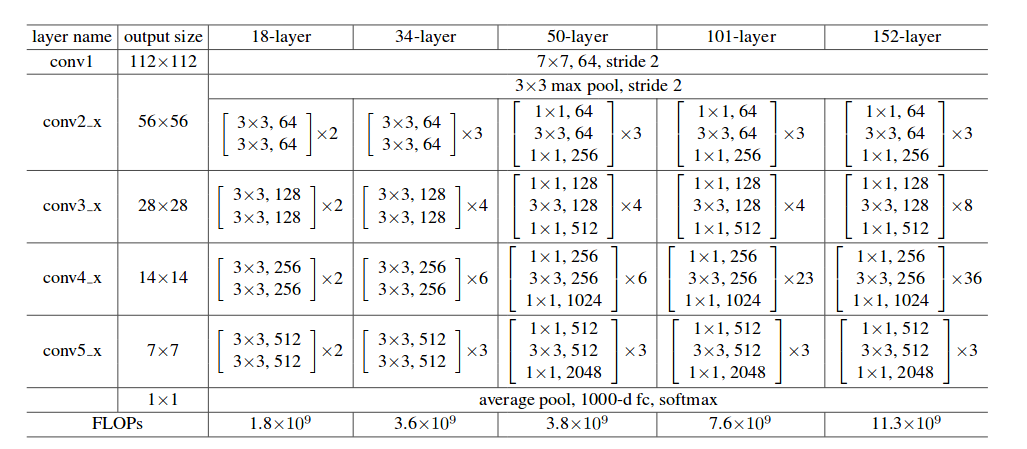
\includegraphics[width=\linewidth]{imgs/resnet_arch.png}
		\caption{resnet50 configuration}%
		\label{fig:resnet conf}
	\end{figure}

	\section[implementation]{Implementation}

	\subsection{Assumptions and Dependencies}%
	\label{sub:Assumptions and Dependencies}
	It is assumed that the MRI scans are collected and processed before feeding
	into the module.

	The program is dependent on external modules and are expected to be
	pre-installed on the system. The modules namely include:

	\begin{itemize}
		\item \href{https://www.fast.ai/}{fast.ai}
		\item \href{https://www.tensorflow.org/}{tensorflow}
		\item \href{https://opencv.org/}{OpenCV}
		\item \href{https://matplotlib.org/}{matplotlib}
	\end{itemize}

	\subsection{Implementation Methods}%
	\label{sub:Implementation Methods}
	After acquiring the data, the data is classified into two classes (binary
	class) of yes, consisting of tumorous cell and no, not consisting tumorous
	cells. A second batch of images is kept separate for prediction, the
	prediction batch.

	Next three machine learning models are created. A \textbf{CNN} or a
	convolutional neural network, \textbf{VGG 16} and \textbf{Resnet 50}. The
	models are implemented in both fast.ai and tensorflow, to be compared later.

	While training the images are resized to $(150 \times 150)$ and augmented at
	runtime, thus removing bias as much as possible. Since there are only two
	possible classes (yes and no), a binary class is sufficient; dividing the
	images into training and testing (validation set) in $80:20$ ratio. Giving
	us $2603 \ \textnormal{and} \ 650$ images for the \textit{yes} and
	\textit{no} classes, respectively.

	After training is complete the models are then evaluated (further discussed
	in Section~\ref{sec:result} )

	\section[result]{Result}%
	\label{sec:result}

	The evaluated models are plotted on graph for better understanding of data.

	\begin{figure}[H]
		\centering
		\subfloat[cnn using tensorflow]
		{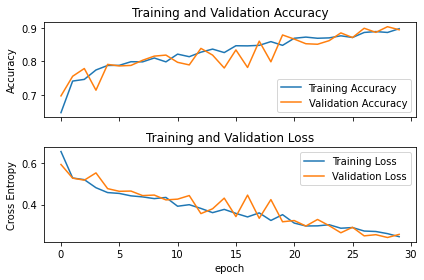
\includegraphics[width=0.4\linewidth]
		{imgs/tf_cnn.png}\label{tf_cnn_cmp}}
		\hspace{0.5cm}
		\subfloat[cnn using fast.ai]
		{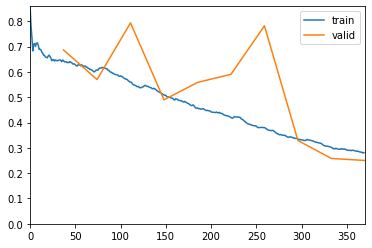
\includegraphics[width=0.5\linewidth]
		{imgs/fastai_cnn.png}\label{fastai_vgg16_cmp}}
		\caption{CNN implemented in fast.ai and tensorflow}
		\label{CNN in fast.ai and tensorflow}
	\end{figure}

	\begin{figure}[H]
		\centering
		\subfloat[vgg16 using tensorflow]
		{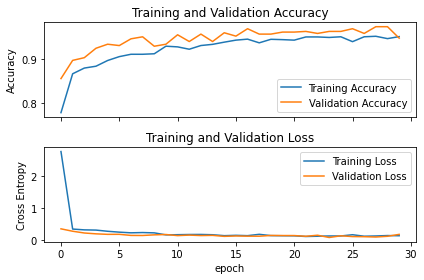
\includegraphics[width=0.4\linewidth]
		{imgs/tf_vgg16.png}\label{tf_vgg16}}
		\hspace{0.5cm}
		\subfloat[vgg16 using fast.ai]
		{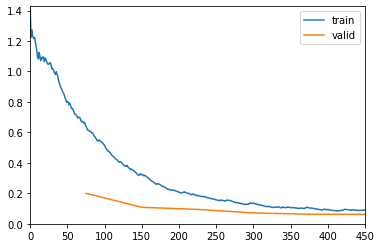
\includegraphics[width=0.5\linewidth]
		{imgs/fastai_vgg16.png}\label{fastai_vgg16}}
		\caption{VGG16 implemented in fast.ai and tensorflow}
		\label{VGG16 in fast.ai and tensorflow}
	\end{figure}


	\begin{figure}[H]
		\centering
		\subfloat[resnet50 using tensorflow]
		{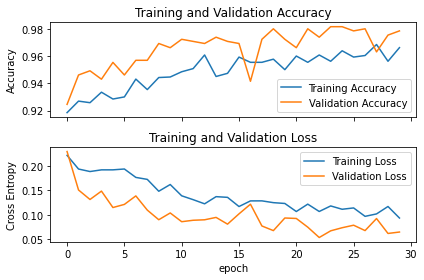
\includegraphics[width=0.4\linewidth]
		{imgs/tf_resnet.png}\label{tf_resnet}}
		\hspace{0.5cm}
		\subfloat[resnet50 using fast.ai]
		{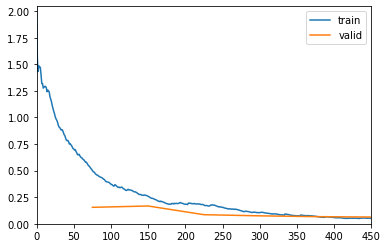
\includegraphics[width=0.5\linewidth]
		{imgs/fastai_resnet.png}\label{fastai_resnet}}
		\caption{Resnet 50 implemented in fast.ai and tensorflow}
		\label{ResNet 50 in fast.ai and tensorflow}
	\end{figure}

	We have achieved around 96\% and 98\% accuracy for for the VGG16 and ResNet,
	respectively; using \textit{tensorflow}, and 97\% (98\% after unfreezing)
	and 97\% (99\% after unfreezing) using \textit{fast.ai}. While using CNN
	accuracy was almost same when implemented by the both the libraries.

	There are lot of room for improvement but due to time and hardware
	constrains we were able to only implement till such.

	\begin{figure}[H]
		\centering
		\subfloat[prediction made by VGG16 implemented in tensorflow]
		{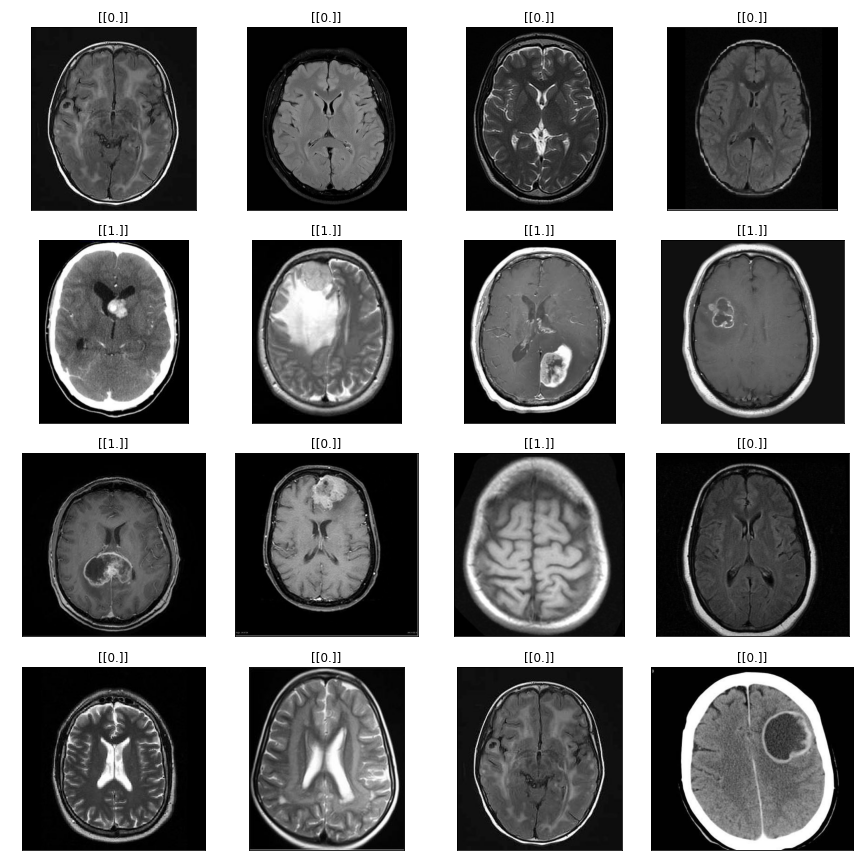
\includegraphics[width=0.5\linewidth]
		{imgs/result.png}\label{vgg16_tf}}
		\hspace{0.3cm}
		\subfloat[prediction made by ResNet50 implemented in fast.ai]
		{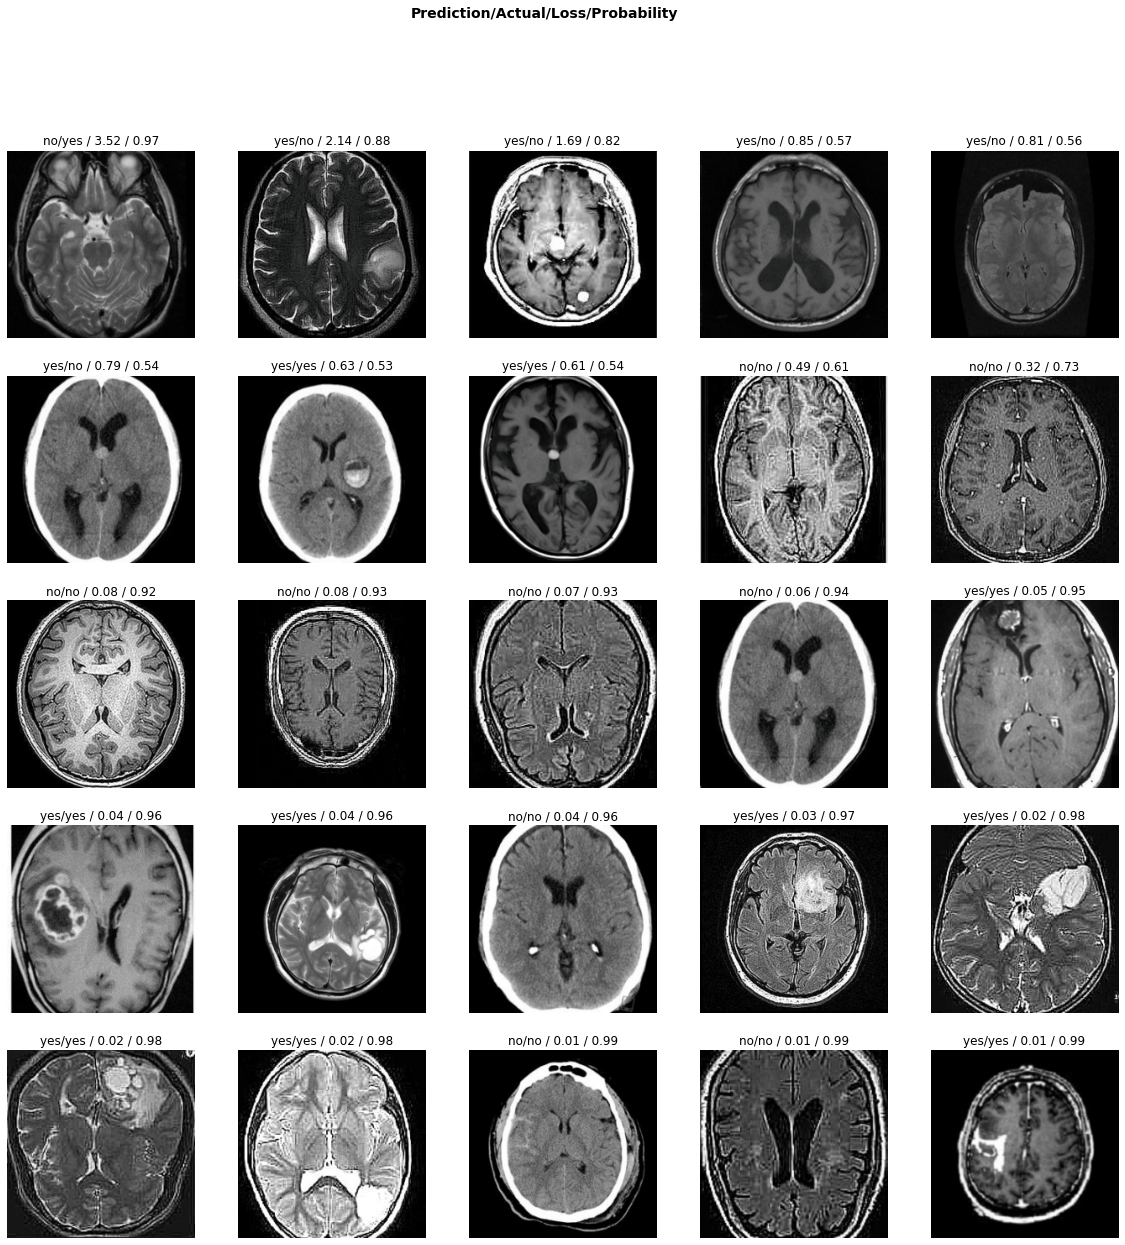
\includegraphics[width=0.5\linewidth]
		{imgs/result_fast_ai.png}\label{resnet_fastai}}
		\caption{Comparing Predictions made by models}
		\label{fig:Results_Comparison}
	\end{figure}

	As it can be seen from Figure~\ref{fig:Results_Comparison} there are some false
	positives in our predictions.

	\section[appendix]{Appendix}%
	\label{sec:Appendix}

	\subsection{Tensorflow Implementation}%
	\label{sub:Tensorflow Implementation}

	\subsubsection{CNN}
	\begin{minted}{python}
import tensorflow as tf
from tensorflow.keras.preprocessing.image import ImageDataGenerator
from tensorflow.keras.models import Sequential
from tensorflow.keras.layers import Flatten, Dropout, Dense
from matplotlib import pyplot as plt

training_dataset_directory = '/content/dataset/training'
testing_dataset_directory = '/content/dataset/testing'

train_datagen = ImageDataGenerator(
    rotation_range=20,
    width_shift_range=0.2,
    height_shift_range=0.2,
    horizontal_flip=True,
    vertical_flip=True,
    rescale=1. / 255,
    fill_mode='nearest',
    validation_split=0.2
)

img_size = (150, 150)
img_shape = img_size + (3,)

training_set = train_datagen.flow_from_directory(
    training_dataset_directory,
    target_size=img_size,
    class_mode='binary',
    subset='training'
)

testing_set = train_datagen.flow_from_directory(
    testing_dataset_directory,
    target_size=img_size,
    class_mode='binary',
    subset='validation'
)

model = tf.keras.models.Sequential()
model.add(
    tf.keras.layers.Conv2D(
        16,
        (3, 3),
        activation='relu',
        input_shape=(150, 150, 3)
    )
)
model.add(
    tf.keras.layers.MaxPool2D(2, 2)
)

model.add(
    tf.keras.layers.Conv2D(
        32,
        (3, 3),
        activation='relu'
    )
)
model.add(
    tf.keras.layers.MaxPool2D(2, 2)
)

model.add(
    tf.keras.layers.Conv2D(
        64,
        (3, 3),
        activation='relu'
    )
)
model.add(
    tf.keras.layers.MaxPool2D(2, 2)
)

model.add(
    tf.keras.layers.Flatten()
)
model.add(
    tf.keras.layers.Dense(
        512,
        activation='relu')
)
model.add(
    tf.keras.layers.Dense(
        1, activation='sigmoid'
    )
)

model.summary()

model.compile(
    optimizer='Adam',
    loss='binary_crossentropy',
    metrics=['accuracy'],
)

history = model.fit(
    training_set,
    epochs=30,
    verbose=1,
    validation_data=testing_set
)
\end{minted}


	\subsubsection{VGG 16}
	\begin{minted}{python}
import tensorflow as tf
from tensorflow.keras.preprocessing.image import ImageDataGenerator
from tensorflow.keras.applications.vgg16 import VGG16, preprocess_input
from tensorflow.keras.models import Sequential
from tensorflow.keras.layers import Flatten, Dropout, Dense
from matplotlib import pyplot as plt

training_dataset_directory = '/content/dataset/training'
testing_dataset_directory = '/content/dataset/testing'

train_datagen = ImageDataGenerator(
    rotation_range=20,
    width_shift_range=0.2,
    height_shift_range=0.2,
    horizontal_flip=True,
    vertical_flip=True,
    preprocessing_function=preprocess_input,
    validation_split=0.2
)

img_size = (150, 150)
img_shape = img_size + (3,)
random_seed = 123

training_set = train_datagen.flow_from_directory(
    training_dataset_directory,
    target_size=img_size,
    class_mode='binary',
    subset='training'
)

testing_set = train_datagen.flow_from_directory(
    testing_dataset_directory,
    target_size=img_size,
    class_mode='binary',
    subset='validation'
)

img_size = (150, 150)
img_shape = img_size + (3,)
random_seed = 123

vgg16 = VGG16(
    weights='imagenet',
    include_top=False,
    input_shape=img_shape
)

num_classes = 1
model = Sequential()
model.add(vgg16)
model.add(Flatten())
model.add(Dense(256, activation='relu'))
model.add(Dropout(0.5))
model.add(Dense(num_classes, activation='sigmoid'))
model.layers[0].trainable = False
model.summary()

model.compile(
    loss='binary_crossentropy',
    optimizer='Adam',
    metrics=['accuracy']
)

epochs = 30
history = model.fit(
    training_set,
    epochs=epochs,
    validation_data=testing_set,
)
\end{minted}


	\subsubsection{ResNet 50}
	\begin{minted}{python}
from tensorflow.keras.preprocessing.image import ImageDataGenerator
from tensorflow.keras.applications.resnet50 import ResNet50, preprocess_input
from tensorflow.keras.models import Sequential
from tensorflow.keras.layers import Flatten, Dropout, Dense
from tensorflow.keras.optimizers import RMSprop, Adam, SGD
from matplotlib import pyplot as plt

training_dataset_directory = '/content/dataset/training'
testing_dataset_directory = '/content/dataset/testing'

train_datagen = ImageDataGenerator(
    rotation_range=20,
    width_shift_range=0.2,
    height_shift_range=0.2,
    horizontal_flip=True,
    vertical_flip=True,
    preprocessing_function=preprocess_input,
    validation_split=0.2
)

img_size = (150, 150)
img_shape = img_size + (3,)
random_seed = 123

training_set = train_datagen.flow_from_directory(
    training_dataset_directory,
    target_size=img_size,
    batch_size=32,
    class_mode='binary',
    subset='training'
)

testing_set = train_datagen.flow_from_directory(
    testing_dataset_directory,
    target_size=img_size,
    class_mode='binary',
    subset='validation'
)

img_size = (150, 150)
img_shape = img_size + (3,)
random_seed = 123

resnet50 = ResNet50(
    weights='imagenet',
    include_top=False,
    input_shape=img_shape
)

num_classes = 1
model = Sequential()
model.add(resnet50)
model.add(Flatten())
model.add(Dense(256, activation='relu'))
model.add(Dropout(0.5))
model.add(Dense(num_classes, activation='sigmoid'))
model.layers[0].trainable = False
model.summary()

model.compile(
    loss='binary_crossentropy',
    optimizer='Adam',
    metrics=['accuracy']
)

epochs = 30
history = model.fit(
    training_set,
    epochs=epochs,
    validation_data=testing_set,
)
\end{minted}


	\subsubsection{Prediction}
	\begin{minted}{python}
import tensorflow as tf
from keras_preprocessing.image import img_to_array
from tensorflow.keras.preprocessing.image import ImageDataGenerator
from tensorflow.keras.applications.resnet50 import preprocess_input, decode_predictions
from tensorflow.keras.preprocessing import image
from tensorflow.keras.preprocessing import image_dataset_from_directory
import matplotlib.image as mpimg
from keras.preprocessing import image
import cv2
import os
import glob

import numpy as np
import matplotlib.pyplot as plt

model = tf.keras.models.load_model('/content/gdrive/MyDrive/model/vgg_imp.h5')

training_dataset_directory = '/content/dataset/training'
testing_dataset_directory = '/content/dataset/testing'

train_datagen = ImageDataGenerator(
    rotation_range=20,
    width_shift_range=0.2,
    height_shift_range=0.2,
    horizontal_flip=True,
    vertical_flip=True,
    preprocessing_function=preprocess_input,
    validation_split=0.2
)

img_size = (150, 150)
img_shape = img_size + (3,)
random_seed = 123

training_set = train_datagen.flow_from_directory(
    training_dataset_directory,
    target_size=img_size,
    class_mode='binary',
    subset='training'
)

testing_set = train_datagen.flow_from_directory(
    testing_dataset_directory,
    target_size=img_size,
    class_mode='binary',
    subset='validation'
)

loss, acc = model.evaluate(training_set)

IMG_SIZE = (150,150)
BATCH_SIZE = 32
new_dataset = image_dataset_from_directory(
    '/content/gdrive/MyDrive/dataset',
    image_size=IMG_SIZE
)

predictions = model.predict(new_dataset,batch_size=BATCH_SIZE)

img_dir = "/content/gdrive/MyDrive/dataset/pred"
data_path = os.path.join(img_dir,'*g')
files = glob.glob(data_path)
data = []
result = []
for f1 in files:
    test_image = image.load_img(f1, target_size = (150, 150))
    test_image = image.img_to_array(test_image)
    test_image = np.expand_dims(test_image, axis = 0)
    images = np.vstack([test_image])
    classes = model.predict(images, batch_size=10)
    classes = np.round(classes)
    data.append(f1)
    result.append(classes)

for x,y in zip(data, result):
  print(x, y)

img = cv2.imread(data[0])
plt.imshow(img)
plt.title(result[0])

L = 4
W = 4
fig, axes = plt.subplots(L, W, figsize = (12,12))
axes = axes.ravel()
for i in np.arange(0, L * W):
    img = cv2.imread(data[i])
    axes[i].imshow(img)
    axes[i].set_title(result[i])
    axes[i].set_xticks([])
    axes[i].set_yticks([])
\end{minted}


	\subsection{fast.ai Implementation}%
	\label{sub:fast.ai Implementation}

	\subsubsection{CNN}
	\begin{minted}{python}
import numpy as np
import pandas as pd
import torch
import keras
import tensorflow as tf
import os
import gc
import pathlib
from keras.models import Sequential
from keras.layers import Conv2D, MaxPooling2D, Flatten, Dense, Dropout, BatchNormalization
from sklearn.metrics import confusion_matrix
from fastai import *
from fastai.vision.all import *
from fastai.tabular.all import *
from fastai.text.all import *
from fastai.vision.data import ImageDataLoaders
from fastai.vision.models import *
import torchvision.models as models
from fastai.callback.schedule import lr_find
from fastai.callback.schedule import *
from matplotlib import pyplot as plt
from fastai.imports import *
from fastai.torch_core import *
from fastai.learner import *
from sklearn.model_selection import train_test_split
from sklearn.preprocessing import OneHotEncoder

print(os.listdir("/content/drive/MyDrive/Colab Notebooks/samples"))
DATA_DIR = "/content/drive/MyDrive/Colab Notebooks/samples/Brain_Tumor"
os.listdir(f'{DATA_DIR}')

data = ImageDataLoaders.from_folder(
    DATA_DIR,
    train=".",
    valid_pct=0.2,
    ds_tfms=aug_transforms(
        mult=2.0,
        do_flip=True,
        flip_vert=True),
    item_tfms=Resize(224),
    bs=64,
    batch_tfms=Normalize.from_stats(
        *imagenet_stats))

data.show_batch(nrows=4, figsize=(10, 10))

model = nn.Sequential(
    nn.Sequential(
        nn.Sequential(
            nn.Conv2d(3, 64, kernel_size=(3, 3),
			stride=(1, 1), padding=(1, 1)), nn.ReLU(inplace=True),
            nn.Conv2d(64, 64, kernel_size=(3, 3),
			stride=(1, 1), padding=(1, 1)), nn.ReLU(inplace=True),
            nn.MaxPool2d(2, stride=2),
            nn.Conv2d(64, 128, kernel_size=(3, 3),
			stride=(1, 1), padding=(1, 1)), nn.ReLU(inplace=True),
            nn.Conv2d(128, 128, kernel_size=(3, 3),
			stride=(1, 1), padding=(1, 1)), nn.ReLU(inplace=True),
            nn.MaxPool2d(2, stride=2),
            nn.Conv2d(128, 256, kernel_size=(3, 3),
			stride=(1, 1), padding=(1, 1)), nn.ReLU(inplace=True),
            nn.Conv2d(256, 256, kernel_size=(3, 3),
			stride=(1, 1), padding=(1, 1)), nn.ReLU(inplace=True),
            nn.MaxPool2d(2, stride=2),
            nn.Conv2d(256, 512, kernel_size=(3, 3),
			stride=(1, 1), padding=(1, 1)), nn.ReLU(inplace=True),
            nn.Conv2d(512, 512, kernel_size=(3, 3),
			stride=(1, 1), padding=(1, 1)), nn.ReLU(inplace=True),
            nn.Conv2d(512, 512, kernel_size=(3, 3),
			stride=(1, 1), padding=(1, 1)), nn.ReLU(inplace=True),
            nn.MaxPool2d(2, stride=2),
        )
    ),
    nn.Sequential(
        AdaptiveConcatPool2d(1),
        nn.Flatten(),
        nn.BatchNorm1d(1024, eps=1e-05, momentum=0.1,
		affine=True, track_running_stats=True),
        nn.Dropout(p=0.25, inplace=False),
        nn.Linear(in_features=1024, out_features=512, bias=False),
        nn.ReLU(),
        nn.BatchNorm1d(512, eps=1e-05, momentum=0.1,
		affine=True, track_running_stats=True),
        nn.Dropout(p=0.5, inplace=False),
        nn.Linear(in_features=512, out_features=2, bias=False)
    )
)

learner = Learner(data, model, metrics=[accuracy, error_rate])

learner.summary()

learner.lr_find()

learner.fit_one_cycle(13, lr_max=slice(1e-3), cbs=[ShowGraphCallback()])

learner.export(
    "/content/drive/MyDrive/Colab Notebooks/pretrained_model/cnn/btc4_final.pkl")

interp = ClassificationInterpretation.from_learner(learner)

interp.plot_top_losses(25, figsize=(20, 20))

interp.plot_confusion_matrix(figsize=(8, 8), dpi=60)
\end{minted}


	\textbf{Prediction}
	\begin{minted}{python}
import numpy as np
import pandas as pd
import fastbook
from fastbook import *
import os
import gc
import pathlib
import fastai.losses
import fastai.layers
from sklearn.metrics import confusion_matrix
from fastai import *
from fastai.vision import *
from fastai.vision.models import *
import torchvision.models as models

learner = load_learner(
    "/content/drive/MyDrive/Colab Notebooks/pretrained_model/cnn/btc4_final.pkl")


def is_true(x):
    if x[0] == 'yes':
        return "Tumor detected."
    else:
        return "Tumor not detected."


img = PILImage.create(
    f"/content/drive/MyDrive/Colab Notebooks/BrainTumor/no/2 no.jpeg")

x = learner.predict(img)

print("Test Result:", is_true(x), "\nProbability:", x[2])
\end{minted}


	\subsubsection{VGG 16}
	\begin{minted}{python}
import numpy as np
import pandas as pd
import torch
import keras
import os
import gc
import pathlib
from sklearn.metrics import confusion_matrix
from fastai import *
from fastai.vision.all import *
from fastai.tabular.all import *
from fastai.text.all import *
from fastai.vision.data import ImageDataLoaders
from fastai.vision.models import *
import torchvision.models as models
from fastai.callback.schedule import lr_find
from fastai.callback.schedule import *
from matplotlib import pyplot as plt
from fastai.imports import *
from fastai.torch_core import *
from fastai.learner import *

print(os.listdir("/content/drive/MyDrive/Colab Notebooks/samples"))
DATA_DIR = "/content/drive/MyDrive/Colab Notebooks/samples/Brain_Tumor"
os.listdir(f'{DATA_DIR}')

data = ImageDataLoaders.from_folder(
    DATA_DIR,
    train=".",
    valid_pct=0.2,
    ds_tfms=aug_transforms(
        mult=1.0,
        do_flip=True,
        flip_vert=True,
        max_warp=0,
        max_rotate=10.0,
        max_zoom=1.1,
        max_lighting=0.2,
        p_affine=0.75,
        mode='bilinear',
        pad_mode='reflection',
        align_corners=True,
        min_scale=1.0),
    item_tfms=Resize(224),
    bs=64,
    val_bs=None,
    num_workers=0,
    batch_tfms=Normalize.from_stats(
        *imagenet_stats))

data.show_batch(nrows=4, figsize=(10, 10))

learner = cnn_learner(
    data, models.vgg16, metrics=[
        accuracy, error_rate], cbs=[
            ShowGraphCallback()], model_dir="/tmp/model/")

learner.lr_find()

learner.model

learner.fit_one_cycle(
    12,
    lr_max=slice(6.918309955e-4),
    cbs=[
        ShowGraphCallback()])

learner.export(
    "/content/drive/MyDrive/Colab Notebooks/pretrained_model/vgg/btc1.pkl")

learner.unfreeze()

learner.lr_find()

learner.fit_one_cycle(
    10,
    lr_max=slice(2.2908675418875646e-6),
    cbs=[
        ShowGraphCallback()])

learner.export(
    "/content/drive/MyDrive/Colab Notebooks/pretrained_model/vgg/final_vgg/btc1_final.pkl")

interp = ClassificationInterpretation.from_learner(learner)

interp.plot_top_losses(25, figsize=(20, 20))

interp.plot_confusion_matrix(figsize=(8, 8), dpi=60)
\end{minted}


	\textbf{Prediction}
	\begin{minted}{python}
import numpy as np
import pandas as pd
import fastbook
from fastbook import *
import os
import gc
import pathlib
import fastai.losses
import fastai.layers
from sklearn.metrics import confusion_matrix
from fastai import *
from fastai.vision import *
from fastai.vision.models import *
import torchvision.models as models

learner = load_learner(
    "/content/drive/MyDrive/Colab Notebooks/pretrained_model/vgg/final_vgg/btc_final.pkl")


def is_true(x):
    if x[0] == 'yes':
        return "Tumor detected."
    else:
        return "Tumor not detected."


img = PILImage.create(
    f"/content/drive/MyDrive/Colab Notebooks/BrainTumor/no/2 no.jpeg")

x = learner.predict(img)

print("Test Result:", is_true(x), "\nProbability:", x[2])
\end{minted}


	\subsubsection{ResNet 50}
	\begin{minted}{python}
import numpy as np
import pandas as pd
import torch
import keras
import os
import gc
import pathlib
from sklearn.metrics import confusion_matrix
from fastai import *
from fastai.vision.all import *
from fastai.tabular.all import *
from fastai.text.all import *
from fastai.vision.data import ImageDataLoaders
from fastai.vision.models import *
import torchvision.models as models
from fastai.callback.schedule import lr_find
from fastai.callback.schedule import *
from matplotlib import pyplot as plt
from fastai.imports import *
from fastai.torch_core import *
from fastai.learner import *

print(os.listdir("/content/drive/MyDrive/Colab Notebooks/samples"))
DATA_DIR = "/content/drive/MyDrive/Colab Notebooks/samples/Brain_Tumor"
os.listdir(f'{DATA_DIR}')

data = ImageDataLoaders.from_folder(
    DATA_DIR,
    train=".",
    valid_pct=0.2,
    ds_tfms=aug_transforms(
        mult=1.0,
        do_flip=True,
        flip_vert=True,
        max_warp=0,
        max_rotate=10.0,
        max_zoom=1.1,
        max_lighting=0.2,
        p_affine=0.75,
        mode='bilinear',
        pad_mode='reflection',
        align_corners=True,
        min_scale=1.0),
    item_tfms=Resize(224),
    bs=64,
    val_bs=None,
    num_workers=0,
    batch_tfms=Normalize.from_stats(
        *imagenet_stats))

data.show_batch(nrows=4, figsize=(10, 10))

learner = cnn_learner(
    data, models.resnet50, metrics=[
        accuracy, error_rate], cbs=[
            ShowGraphCallback()], model_dir="/tmp/model/")

learner.lr_find()

learner.model

learner.fit_one_cycle(6, lr_max=slice(8.32e-4), cbs=[ShowGraphCallback()])

learner.export(
    "/content/drive/MyDrive/Colab Notebooks/pretrained_model/resnet/btc2.pkl")

learner.unfreeze()

learner.lr_find()

learner.fit_one_cycle(
    6,
    lr_max=slice(5.754399353463668e-6),
    cbs=[
        ShowGraphCallback()])

learner.fit_one_cycle(4, lr_max=slice(2.7e-5), cbs=[ShowGraphCallback()])

learner.fit_one_cycle(4, lr_max=slice(2.9e-5), cbs=[ShowGraphCallback()])

learner.export(
    "/content/drive/MyDrive/Colab Notebooks/pretrained_model/resnet/final_resnet/btc_final2.pkl")

interp = ClassificationInterpretation.from_learner(learner)

interp.plot_top_losses(25, figsize=(20, 20))

interp.plot_confusion_matrix(figsize=(8, 8), dpi=60)
\end{minted}


	\textbf{Prediction}
	\begin{minted}{python}
import numpy as np
import pandas as pd
import fastbook
from fastbook import *
import os
import gc
import pathlib
import fastai.losses
import fastai.layers
from sklearn.metrics import confusion_matrix
from fastai import *
from fastai.vision import *
from fastai.vision.models import *
import torchvision.models as models

learner = load_learner(
    "/content/drive/MyDrive/Colab Notebooks/pretrained_model/vgg/final_vgg/btc_final.pkl")


def is_true(x):
    if x[0] == 'yes':
        return "Tumor detected."
    else:
        return "Tumor not detected."


img = PILImage.create(
    f"/content/drive/MyDrive/Colab Notebooks/BrainTumor/no/2 no.jpeg")

x = learner.predict(img)

print("Test Result:", is_true(x), "\nProbability:", x[2])
\end{minted}


	\emergencystretch=1em
	\printbibliography[heading=bibintoc,title={References}]

\end{document}
